\documentclass[
  bibliography=totoc,     % Literatur im Inhaltsverzeichnis
  captions=tableheading,  % Tabellenüberschriften
  titlepage=firstiscover, % Titelseite ist Deckblatt
]{scrartcl}

% Paket float verbessern
\usepackage{scrhack}

% Warnung, falls nochmal kompiliert werden muss
\usepackage[aux]{rerunfilecheck}

% unverzichtbare Mathe-Befehle
\usepackage{amsmath}
% viele Mathe-Symbole
\usepackage{amssymb}
% Erweiterungen für amsmath
\usepackage{mathtools}

% Fonteinstellungen
\usepackage{fontspec}
% Latin Modern Fonts werden automatisch geladen
% Alternativ zum Beispiel:
%\setromanfont{Libertinus Serif}
%\setsansfont{Libertinus Sans}
%\setmonofont{Libertinus Mono}

% Wenn man andere Schriftarten gesetzt hat,
% sollte man das Seiten-Layout neu berechnen lassen
\recalctypearea{}

% deutsche Spracheinstellungen
\usepackage[ngerman]{babel}


\usepackage[
  math-style=ISO,    % ┐
  bold-style=ISO,    % │
  sans-style=italic, % │ ISO-Standard folgen
  nabla=upright,     % │
  partial=upright,   % ┘
  warnings-off={           % ┐
    mathtools-colon,       % │ unnötige Warnungen ausschalten
    mathtools-overbracket, % │
  },                       % ┘
]{unicode-math}

% traditionelle Fonts für Mathematik
\setmathfont{Latin Modern Math}
% Alternativ zum Beispiel:
%\setmathfont{Libertinus Math}

\setmathfont{XITS Math}[range={scr, bfscr}]
\setmathfont{XITS Math}[range={cal, bfcal}, StylisticSet=1]

% Zahlen und Einheiten
\usepackage[
  locale=DE,                   % deutsche Einstellungen
  separate-uncertainty=true,   % immer Unsicherheit mit \pm
  per-mode=symbol-or-fraction, % / in inline math, fraction in display math
]{siunitx}

% chemische Formeln
\usepackage[
  version=4,
  math-greek=default, % ┐ mit unicode-math zusammenarbeiten
  text-greek=default, % ┘
]{mhchem}

% richtige Anführungszeichen
\usepackage[autostyle]{csquotes}

% schöne Brüche im Text
\usepackage{xfrac}

% Standardplatzierung für Floats einstellen
\usepackage{float}
\floatplacement{figure}{htbp}
\floatplacement{table}{htbp}

% Floats innerhalb einer Section halten
\usepackage[
  section, % Floats innerhalb der Section halten
  below,   % unterhalb der Section aber auf der selben Seite ist ok
]{placeins}

% Seite drehen für breite Tabellen: landscape Umgebung
\usepackage{pdflscape}

% Captions schöner machen.
\usepackage[
  labelfont=bf,        % Tabelle x: Abbildung y: ist jetzt fett
  font=small,          % Schrift etwas kleiner als Dokument
  width=0.9\textwidth, % maximale Breite einer Caption schmaler
]{caption}
% subfigure, subtable, subref
\usepackage{subcaption}

% Grafiken können eingebunden werden
\usepackage{graphicx}

% schöne Tabellen
\usepackage{booktabs}

% Verbesserungen am Schriftbild
\usepackage{microtype}

% Literaturverzeichnis
\usepackage[
  backend=biber,
]{biblatex}
% Quellendatenbank
\addbibresource{lit.bib}
\addbibresource{programme.bib}

% Hyperlinks im Dokument
\usepackage[
  german,
  unicode,        % Unicode in PDF-Attributen erlauben
  pdfusetitle,    % Titel, Autoren und Datum als PDF-Attribute
  pdfcreator={},  % ┐ PDF-Attribute säubern
  pdfproducer={}, % ┘
]{hyperref}
% erweiterte Bookmarks im PDF
\usepackage{bookmark}

% Trennung von Wörtern mit Strichen
\usepackage[shortcuts]{extdash}

\author{%
  Benjamin Schäfer\\%
  \href{mailto:benjamin.schaefer@tu-dortmund.de}{leander.flottau@tu-dortmund.de}%
  \and%
  Jan Gaschina\\%
  \href{mailto:jan.gaschina@tu-dortmund.de}{jan.gaschina@tu-dortmund.de}%
}
\publishers{TU Dortmund – Fakultät Physik}


\subject{V27}
\title{Der Zeeman-Effekt}
\date{%
  Durchführung: 12.01.2022
  \hspace{3em}
  Abgabe: 28.01.2022
 \hspace{3em}
 Korrektur: 10.02.2022
}

\begin{document}

\maketitle
\thispagestyle{empty}
\tableofcontents
\newpage
\section{Zielsetzung}
In diesem Versuch sollen die Eigenschaften des HeNe-Lasers untersucht werden. Zu diesen Eigenschaften zählt
neben der Wellenlänge und der Polarisation auch das TE-Modenspektrum. Zudem soll die Stabilitätsbedingung 
unter änderung der Resonatorlänge und der Resonatorspiegel überprüft werden.

\section{Theorie}
\label{sec:Theorie}
In diesem Kapitel sollen kurz die theoretischen Grundlagen des HeNe-Lasers erleutert werden.

\subsection{Aufbau und Funktion eines Lasers}
\label{sec:aufbauUndFunktion}
Das Wort Laser ist ein Akronym und steht für Light Amplification by Stimulated Emission of Radiation.
Jeder Laser besteht aus einem optischen Resonator, einem verstärkendem Medium und einer Energiepumpe.
Der optische Resonator besteht an sich aus zwei gegenüberliegenden, hochreflektiven Spiegeln von 
denen mindestens einer halbdurchlässig ist. Die Spiegel können sowohl planar als auch konkav gebaut sein.
Zwischen den Siegeln, also inneralb des optischen Resonators befindet sich das verstärkende Medium. Hier 
wird das Laserlicht sowohl erzeugt als auch durch die später noch erklärte stimmulierte Emmission
verstärkt. Beim Helium-Neon-Laser ist das verstärkende Medium das Neon. Da das Experiment bei Raumtemperatur 
unter nicht zu hohen Drücken durchgeführt wird, liegt es wie auch das Helium als Gas in einem Kapilarrohr vor.
Das letzte zur Funktion nötige Element ist die Energiepumpe, sie liefert die Energie nach welche über das 
ausfallende Laserlicht und an diversen anderen Stellen aus dem System entkommt. Im Fall des HeNe-Lasers
ist das Helium die Energiepumpe. Es wird durch zwei Elektroden an welchen eine Hochspannung anliegt
auf einen höheres Energieniveau gebracht und gibt seine Energie dann später über thermische Stöße an das 
Neon ab. Der Laser funktioniert also dadurch das Neon durch das angeregte Helium auf einen höheren 
Energiezustand gebracht wird, das Neon beginnt zu leuchten. Kohärent und linear polarisiert wird das Licht
durch den Resonator und Brewsterfenster.

\subsection{Brewsterfenster}
\label{sec:Brewsterfenster}
Die Brewsterfenster sind ein optionales Bauteil, werden in diesem Versuch jedoch verwendet.
Sie bestehen aus planparallelen Glaspaltten welche zur Strahlachse im Brewsterwinkel angeordnet sind.
Sie reflektieren das senkrecht zur Einfallsebene polarisierte Licht und lassen das parallel polarisierte 
Licht vollständig durch. Dadurch wird die senkrechte polarisation stark unterdrückt.

\subsection{Emmission und Absorbtion}
\label{sec:EmmissionUndAbsorbtion}
Zunächst wird ein System betrachtet welches nur zwei Energiezustände, $n_1$ und $n_2$ kennt.
Es gibt nun drei mögliche Prozesse welchen einen wechsel des Energiezustandes zur folge haben.
Der erste ist die Absorbtion. Das System absorbiert ein Energiequant und gelangt so vom nicht 
angeregten Zustand $n_1$ in den angeregten Zustand $n_2$. Der zweite Prozess ist die spontane
Emmission. Hier befindet sich das System zunächst in $n_2$ und fällt dann zu einem unbestimmten 
Zeitpunkt unter Emmission eines in Raumrichtung und Phase unbestimmten Energiequants auf $n_1$ zurück.
Der dritte und für den Laser entscheidende Prozess ist die stimmulierte Emmission. Hier befindet sich 
das System ebenfalls in $n_2$ wird dann aber von einem Photon getroffen und fällt unter Emmission
eines dem einfallenden Photon in Raumrichtung und Phase gleichenden Photons zurück auf $n_1$. Dieser letzte
Prozess führt dazu das dass Laserlicht nur in Richtung der Strahlachse verstärkt wird, kohärent ist, und
falls Brewsterfenster verwendet werden, auch linear polarisiert ist. Die einfallenden Energiequante müssen 
energetisch jeweils dem Energieunterschied von $n_1$ und $n_2$ entsprechen.


\section{Fehler}
\label{sec:Fehler}
Der Mittelwert:
\begin{center}
  \begin{equation}
    \label{eq:Mittelwert}
  \bar{x} = \frac{1}{n} \sum \nolimits_{i=0} x_i
  \end{equation} 
\end{center}

Die Standardabweichung:
\begin{center}
  \begin{equation}
    \label{eq:standardabweichung}
    \sigma=\sqrt{\frac{\sum(x_i-\bar{x})^2}{n-1}}
  \end{equation}
\end{center}

Der Fehler des Mittelwertes:
\begin{center}
  \begin{equation}
    \label{eq:mittelwertfehler}
    \sigma_{\bar{x}}=\frac{\sigma}{\sqrt{n}}
  \end{equation}

  
\end{center}

%Die Poissonverteilung:
%\begin{center}
%    \begin{equation}
%        \label{eq:poisson}
%        \Delta N=\sqrt{N}
%        \end{equation}
%\end{center}

Die Gaußsche Fehlerfortpflanzung:
\begin{center}
\begin{equation}
  \label{eq:gaussfehler}  
\sigma_x=\sqrt{(\frac{\partial f}{\partial x_1})^2\sigma_{x_1}^2+(\frac{\partial f}{\partial x_2})^2\sigma_{x_2}^2+...+(\frac{\partial f}{\partial x_n})^2\sigma_{x_n}^2}
\end{equation}
\end{center}

Die Prozentuale Abweichung:

\begin{center}
  \begin{equation}
    \label{eq:prozentuale} 
    Abweichung=\frac{\mathrm{Experimenteller Wert - Theoriewert}}{\mathrm{Theoriewert}}\times 100 
   \end{equation}
  \end{center}
\section{Durchführung}
\label{sec:Durchfuehrung}
In diesem Kapitel sollen die einzelnen Schritte des Versuches erklärt werden.
\subsection{Ausrichtung und Start des Laserbetriebs}
\label{sec:ausrichtung}
Um den Laser zur Funktion zu bringen müssen alle Komponenten nach einer Strahlachse ausgerichtet werden.
Dazu wird ein grüner Hilfslaser am einen ende der optischen Bank eingeschaltet und auf ein Fadenkreuz 
am anderen Ende ausgerichtet. Nun werden nacheinander das Laserrohr und die Resonatorspiegel auf der
Bank arretiert und so ausgerichtet das die entsprechenden Beugungsringe und Reflexe wieder ins Fadenkreuz 
treffen. Die Resonatorspiegel werden dazu zunächst sehr nah an den Enden des Laserrohres montiert.
Sobald alle komponenten gut ausgerichtet sind wird der grüne Laser abgeschaltet und die Pumpspannung des 
HeNe-Lases eingeschaltet. Das Laserrohr beginnt nun rötlich zu leuchten. Nach kurzem nachstellen der 
Resonatorspiegel stellt sich der Laserbetrieb ein was an einem roten Lichtpunkt im Fadenkreuz zu erkennen ist.

\subsection{Überprüfung der Stabilitätsbedingung}
\label{sec:stabilitaetsbedingung}
Um die Stabilitätsbedingung zu überprüfen wird zunächst die von den Resonatorspiegel abhängige maximale 
Länge berechnet unter welcher der Laser noch stabil läuft. Im Anschluss daran werden die beiden Spiegel 
schrittweise voneinander entfernt und immer wieder neu ausgerichtet um den Laserbetrieb aufrecht zu erhalten.
Dabei wird jedes mal mit Hilfe einer Photodiode die maximale Leistung eingestellt.
Wenn der Laserbetrieb bei der maximal möglichen Länge noch aufrecht erhalten werden kann ist die 
Stabilitätsbedingung sicher erfüllt. Dies wird mit zwei verschiedenen Spiegeln durchgeführt.

\subsection{Beobachtung von TEM-Moden}
\label{sec:temmoden}

\subsection{Bestimmung der Polarisation}
\label{sec:polarisation}
Um die Polarisation des Laserlichtes zu vermessen wid ein drehbahrer Polarisationsfilter in den Strahlweg 
gebracht. Hinter dem Polarisationsfilter wird wieder dei Photodiode positioniert. Nun wird der
Polarisationsfilter in kleinen Schritten gedreht und nach jeder Drehung die Intensität gemessen.

\subsection{Frequenzspektrum}
\label{sec:Frequenzspektrum}
Der Laser wird bei unterschiedlichen Resonatorlängen auf eine zeitlich hochauflösende Photodiode gerichtet.
Die Photodiode ist an einen Spektrum-Analyzer angeschlossen. Hier können die Frequenzen der entstehenden 
Schwebungen als Peaks abgelesen werden.

\subsection{Bestimmung der Wellenlänge}
\label{sec:wellenlaenge}
Um die Wellenlänge des Lasers zu bestimmen wid in den Strahlgang des Lasers ein optisches Gitter gestellt.
Auf einem Schirm können nun als Resultat der Frauenhoferbeugung mehere Strahlungsmaxima beobachtet werden.
Aus ihren Abständen kann die Wellenlänge des Laseers berechnet werden.



\section{Auswertung}
\label{sec:auswertung}

In diesem Kapitel werden die aufgenommenen Messwerte ausgewertet.




\subsection{Schwingungsmoden und Bandbreite}
\label{sec:schwingungsmoden}

In diesem Abschnitt wurden drei aufeinanderfolgende Schwingungsmoden des Klystrons vermessen und graphisch dargestellt.
Ausserdem wurde die Bandbreite einer Mode vermessen und daraus die elektronische Bandbreite errechnet.
Die Messwerte zu den verschiedenen Reflektorspannungen sind in \autoref{tab:schwingmod} zu finden und wurden in vielfachem der maximal gemessenen Leistung angegeben, da ultimativ nur die Lage zueinander interessiert und es so leichter vergleichbar ist.


\begin{table}
\centering
\caption{Schwingungsmoden für verschiedene Reflektorspannungen}
\begin{tabular}{c c}
\toprule
{$V$[V]} & {$P/P_{\text{max}}$}\\
\midrule
220&	0,833\\
210	&0\\
230	&0\\
\midrule
140	&1\\
130	&0\\
150	&0\\
\midrule
80	&0,777\\
70	&0\\
90	&0\\
\bottomrule
\label{tab:schwingmod}
\end{tabular}
\end{table}



Zur graphischen Darstellung wurde für jede Mode eine Parabel an die Messwerte gefittet. Diese hat die Form:


\begin{equation}
P(V) = m\cdot (V - V_0)^2 + P_0
\label{eq:parabel}
\end{equation}

Die sich ergebenden Werte sind in \autoref{tab:schwingmod2} zu sehen. Für die Messwerte der Leistung wurde ein Fehler in der Größenordnung der letzten Nachkommastelle angenommen und dann genauso skaliert wie die Werte selbst ($P_{\text{Fehler}}/P_{\text{max}}$), um dimensionslos zu sein.

\begin{table}
\centering
\caption{Parameterwerte der Parabelfits}
\begin{tabular}{c c c}
\toprule
{$V_0$[V]} & {$P_0$} & {$m$[1/V]}\\
\midrule
{220,0000 \pm 0,2547}  & { 0,8330 \pm 0,0600} & {-0,0083 \pm 0,0007}\\
{140,0000 \pm 0,2121}  &  {1,0000 \pm 0,0600} & {-0,0100 \pm 0,0007}\\
{80,0000 \pm 0,2730}  &  {0,7770  \pm 0,0600} & {-0,0078 \pm 0,0007}\\
\bottomrule
\label{tab:schwingmod2}
\end{tabular}
\end{table}



Die Messwerte und sich ergebende Parabeln sind in \autoref{fig:schwingmod} dargstellt.

\begin{figure}
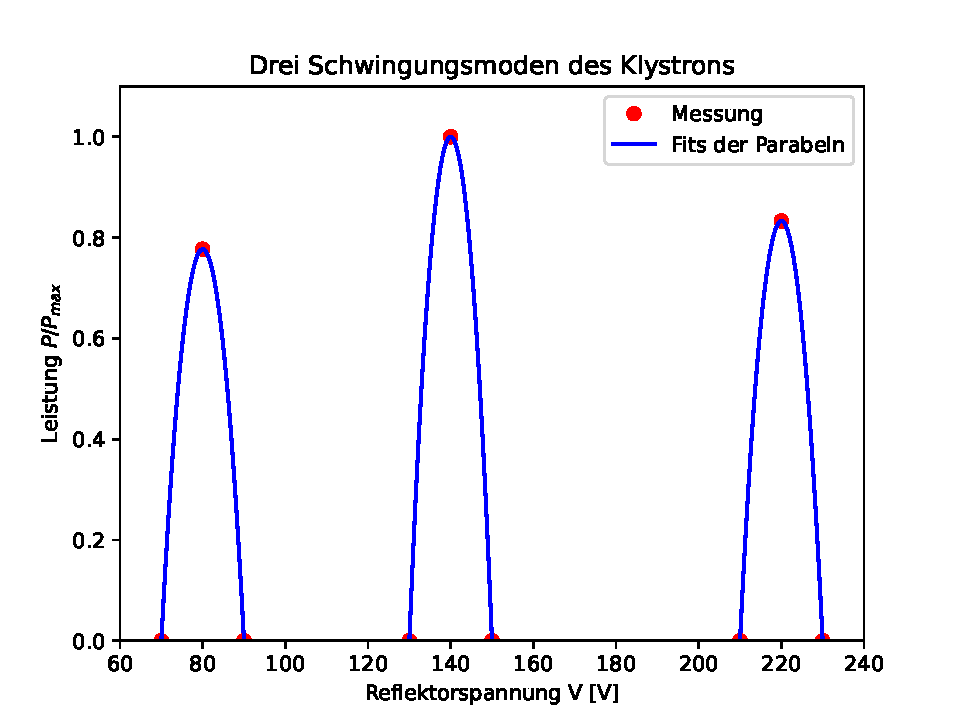
\includegraphics{figures/Schwingungsmoden.pdf}
\caption{Messwerte und Parabeln dreier Schwingungsmoden des Klystrons}
\label{fig:schwingmod}
\end{figure}


Die Messung zur Bandbreite einer Mode ist in \autoref{tab:bandbreite} zu finden. Für die Messwerte der Frequenz wurde eine Unsicherheit der Größe $0,5\,$MHz und für die Messwerte der Spannung eine Unsicherheit von $10\,$V angenommen.

\begin{table}
\centering
\caption{Messwerte zur Bestimmung der Bandbreite}
\begin{tabular}{c c}
\toprule
{$V$[V]} & {$f$[MHz]}\\
\midrule
220 & 9014\\
210&8999\\
230&9029\\
\bottomrule
\label{tab:bandbreite}
\end{tabular}
\end{table}


Die elektronische Bandbreite $B$ und Abstimmempfindlichkeit $E$ ergaben sich zu:

\begin{equation}
B = (30 \pm 0,707)\,\text{MHz}
\label{eq:bandbreite}
\end{equation}
\begin{equation}
E = (1,5 \pm 1,061) \frac{\text{MHz}}{\text{V}}
\label{eq:elbandbreite}
\end{equation}

Unsicherheiten wurden dabei mittels Gaußscher Fehlerfortpflanzung berechnet.

 







\subsection{Frequenz, Wellenlänge und Dämpfung}
\label{sec:fwd}


In diesem Abschnitt wird die Messung zur Bestimmung der Wellenlänge und der Frequenz der Mikrowellenstrahlung ausgewertet, sowie die, auf dem Dämpfungsglied angegebene Dämpfung, mit Messwerten verglichen.
Die gemessenen Positionen zweier aufeinanderfolgender Minima der stehenden Welle mit direkt gemessener Frequenz $f$ sind in \autoref{tab:minima} zu finden.


\begin{table}
\centering
\caption{Positionen zweier aufeinanderfolgender Minima}
\begin{tabular}{c c c}
\toprule
{$f$[MHz]} & {1. Minimum [mm]}&{2. Minimum [mm]}\\
\midrule
{9014\pm0,5}&{62,6\pm0,05}&{87,9\pm0,05}
\bottomrule
\label{tab:minima}
\end{tabular}
\end{table}

Die Wellenlänge $\lambda_g$ ergibt sich aus dem doppelten des Abstands der Minima aus \autoref{tab:minima} zu:

\begin{equation}
\lambda_g = (50,6 \pm 0,141)\,\text{mm}
\label{eq:wellenlaenge}
\end{equation}

Alle Fehler in diesem Abschnitt wurden mittels Gaußscher Fehlerfortpflanzung ermittelt.
Die Frequenz $f$ lässt sich berechnen über folgende Formel:

\begin{equation}
f = c\cdot\sqrt{ (\frac{1}{\lambda_g})^2 + (\frac{1}{2a})^2 }
\label{eq:freq}
\end{equation}

Die Innenabmessung $a = (22,860 \pm 0,046)\,$mm des Hohlraumleiters und die Lichtgeschwindigkeit $c = 3\cdot 10^{11} \frac{\text{mm}}{\text{s}}$ wurden dabei der Versuchsanleitung entnommen.
Daraus ergibt sich die Frequenz zu:

\begin{equation}
f = (8843,47 \pm 14,79)\,\text{MHz}
\label{eq:freq2}
\end{equation}

Die Messwerte zur Dämpfung des Dämpfungsglied sind in \autoref{tab:daempf} zu sehen.


\begin{table}
\centering
\caption{Messwerte zur Dämpfung des Dämpfungsgliedes}
\begin{tabular}{c c c}
\toprule
{Mikrometereinstellung [mm]} & {gemessene Dämpfung [dB]} & {Dämpfung laut Eichkurve [dB]}\\
\midrule
3,00	&0	&16
3,18	&2	&19
3,31	&4	&20
3,59	&6	&24
3,70	&8	&25
3,89	&10	&29

\bottomrule
\label{tab:daempf}
\end{tabular}
\end{table}

Zur besseren Auswertbarkeit wurde danach die Dämpfungswerte aus der Eichkurve auf den ersten Messwert bezogen nach der Formel:

\begin{equation}
\text{Dämpfung}(x)_{\text{dB}} = x - 16\,\text{dB}
\label{eq:daempf}
\end{equation}

Die Dämpfungen in Abhängigkeit der Mikrometereinstellung sind in \autoref{fig:daempf} dargestellt.



\begin{figure}
\includegraphics{figures/Dämpfungsglied.pdf}
\caption{Gemessene und angegebene Dämpfungskurve}
\label{fig:daempf}
\end{figure}










\subsection{Stehwellenverhältnis}
\label{sec:welligkeit}


In diesem Abschnitt wird das Stehwellenverhältnis $S$, auch Welligkeit genannt, für verschiedene Sondentiefen und mit verschiedenen Messmethoden bestimmt.
Die direkte Messung der Welligkeit mittels des SWR-Meters für verschiedene Sondentiefen ist in \autoref{tab:swr} zu sehen.


\begin{table}
\centering
\caption{Direkt abgelesenes Stehwellenverhältnis $S$ am SWR-Meter}
\begin{tabular}{c c}
\toprule
{Sondentiefe [mm]} & {S}\\
\midrule
3&1,16\\
5&1,55\\
7&3,50\\
9&nicht ablesbar\\
\bottomrule
\label{tab:swr}
\end{tabular}
\end{table}


Die Messung zur 3\,dB-Methode ist in \autoref{tab:3db} zu finden. Die Werte $d_1$ und $d_2$ geben die Stellen an, an denen der Ausschlag des SWR-Meters um 3\,dB größer war als am dazu naheliegendsten Minimum. Der Abstand zweier aufeinanderfolgender Minima ist auch eingetragen, um daraus wie in \autoref{sec:fwd} die Wellenlänge $\lambda_g$ zu brechnen.



\begin{table}
\centering
\caption{SWR-Meter Einstellungen zur Bestimmung der Welligkeit mittels der 3\,dB Methode}
\begin{tabular}{c c c c}
\toprule
{$d_1$ [mm]} & {$d_2$ [mm]}& {1.Minimum [mm]}& {2. Minimum [mm]}\\
\midrule
91,20 & 89,50 & 103,00 & 78,90\\
\bottomrule
\label{tab:3db}
\end{tabular}
\end{table}

Das Stehwellenverhältnis lässt sich mittels folgender Formel berechnen:

\begin{equation}
S = \frac{\lambda_g}{\pi (d_1 - d_2)}
\label{eq:welligkeit1}
\end{equation}

Für die Unsicherheiten der Entfernungsmessung wurden $0,005$\,mm angenommen. Damit berechnet sich das Stehwellenverhältnis zu:

\begin{equation}
S = 9,025 \pm 0,038
\label{eq:welligkeit2}
\end{equation}

bei einer Sondentiefe von 9\,mm. Alle Unsicherheiten wurden in diesem Abschnitt mittels Gaußscher Fehlerfortpflanzung berechnet.\\
Die Messdaten für die Abschwächer-Methode sind in \autoref{tab:abschw} zu finden.


\begin{table}
\centering
\caption{Am Dämpfungsglied eingestellte Dämpfungen $A_1$ bzw $A_2$ zur Abschwächer-Methode}
\begin{tabular}{c c c c}
\toprule
{$A_1$ [dB]} & {$A_2$ [dB]}\\
\midrule
20 & 42
\bottomrule
\label{tab:abschw}
\end{tabular}
\end{table}

Das Stehwellenverhältnis lässt sich mit \autoref{eq:abschw} berechnen.

\begin{equation}
S = 10^{\frac{A_2 - A_1}{20}}
\label{eq:abschw}
\end{equation}

Es ergibt sich der Wert:

\begin{equation}
S = 12,589 \pm 2,0497
\label{eq:abschw2}
\end{equation}

Die Unsicherheit der Dämpfung wurde hierbei zu 1\,dB angenommen.








































\section{Diskussion}
\label{sec:Diskussion}

Dieses Kapitel befasst sich mit der Diskussion der im \autoref{sec:auswertung} erhaltenen Ergebnisse.



Der Fit einer Parabel an die Messwerte der drei Schwingungsmoden aus \autoref{sec:schwingungsmoden}, wie sie in \autoref{fig:schwingmod} graphisch dargestellt ist, deckt sich sehr gut mit den Messwerten.
Die Scheitelpunkte der Parabeln liegen für kleinere Reflektorspannungen dichter beieinander, aber die größten Werte werden nicht kleiner zu niedrigeren Reflektorspannungen.
Dies kann an unsachgemäßem Ablesen der Leistung am Oszilloskop liegen, aber auch auftretenden Resonanzen innerhalb des Zusammenspiels aus Messapparaturen, die hierfür verwendet wurden.\\
Die Messung der Bandbreite war mit großen Unsicherheiten behaftet, welche vorallem bei der Abstimmempfindlichkeit sichtbar werden.
Für die Abstimmempfindlichkeit $E$ ergab sich der Wert zu:

\begin{equation}
E = (1,5 \pm 1,061) \frac{\text{MHz}}{\text{V}}
\label{eq:elbandbreite2}
\end{equation}

Die relative Unsicherheit beträgt somit ca 71\%. Dies lässt sich durch mehrere Effekte erklären. Zum einen handelt es sich hierbei um eine Einzelmessung.
Für genauere Werte sollte mehrfach gemessen und daraus der Mittelwert berechnet werden.
Zum anderen waren die Flanken der Schwingungsmode sehr viel steiler als bei einer der Parabeln, wie sie in \autoref{fig:schwingmod} zu sehen sind.
Der größte Faktor war jedoch, dass sich die Reflektorspannung nur auf 10\,V genau bestimmen ließ.\\

In \autoref{sec:fwd} wurde die Wellenlänge der verwendeten Strahlung zu $\lambda_g = (50,6 \pm 0,141)$\,mm bestimmt. Diese liegt in dem Bereich, der als Mikrowellenstrahlung bezeichnet wird.
Die Frequenz $f$ wurde auf zwei Arten bestimmt. Einmal direkt per Messung mit einem Frequenzmessgerät und einmal indirekt über die Wellenlänge und Maße des Hohlleiters.\\
Die erste Messung ergab eine Frequenz von $f = (9014 \pm 0,5)$\,MHz und die zweite $f = (8843,47 \pm 14,79)$\,MHz.
Der zweite Wert hat eine deutlich größere Unsicherheit und unterscheidet sich vom ersten um etwa 1,9\% des ersten Wertes.
Unter der Annahme, dass die erste Messmethode deutlich näher an dem realen Wert liegt, kann das Ergebnis der Zweiten auch als recht genau betrachtet werden.\\
In \autoref{fig:daempf} sind die gemessene und die Eichkurve des Dämpfungsgliedes zu sehen. 

Die Messreihe wurde bei 16,dB anstelle von 0,dB gestartet, da dort die Eichkurve des Dämpfungsgliedes leichter ablesbar war.
Der maximale Unterschied zwischen gemessener Dämpfung und abgelesener Betrug 3/,dB.
Da auch das Ablesen der Dämpfung auf der Eichkurve mit Unsicherheiten in der Größenordnung von einigen dB behaftet ist, lässt sich sagen, dass die beiden Kurven gut übereinstimmen.
Das direkte Messen der Welligkeit mittels eines SWR-Meters ist nur  für geringe Welligkeiten möglich.
Dies hat praktische Gründe:
So kommt das Messen von Welligkeiten häufig dort vor, wo stehende Wellen vermieden werden sollen und somit nur sehr geringe Welligkeiten akzeptabel sind.
Bei einer Sondentiefe von 9/,mm war somit kein Wert für das Stehwellenverhältnis mehr ablesbar.

Zur Bestimmung dieses Wertes wurden zwei verschiedene Methoden verwendet.
Bei der 3,dB-Methode ging neben den Messwerten bestimmter Stellen der Welle auch die Wellenlänge mit ein, welche selbst eine fehlerbehaftete Größe war.
Die Welligkeit ist jedoch nur proportional bzw antiproportional zu den gemessenen Werten.
Dahingegen weist die Welligkeit bei der Abschwächer-Methode einen exponentiellen Zusammenhang zu den Messwerten auf.
Dieser exponentielle Zusammenhang ist die Ursache dafür, dass kleine Schwankungen der Messwerte zu großen Schwankungen des berechneten Stehwellenverhältnisses führen und damit womöglich auch die Ursache für den großen Unterschied von ca 28\% der Ergebnisse beider Methoden.
Der durch die 3,dB-Methode erhaltene Wert $S = 9,025 \pm 0,038$ ist der genauere.

\section{Literatur}
[1] Versuchsanleitung, Philips, Experimente mit Mikrowellen 1


























\printbibliography{}

\end{document}
